\documentclass[../main.tex]{subfiles}
\graphicspath{{\subfix{../figures/}}}

\begin{document}
\section{里氏代换原则(LSP)}
Liskov Substitution Principle

\noindent 1988年,由麻省理工的Barbara Liskov提出,其思想表达为:
如果对每一个类型为T1的对象o1,都有类型为T2的对象o2,使得以T1定义的所有程序P在所有的对象o1都代换成o2时,程序P的行为没有变化,那么类型T2是类型T1的子类型.

\noindent 里氏代换原则是继承复用的基石.只有当派生类可以替换掉基类,软件功能不会受到影响,基类才能真正被复用,而派生类也才能够在基类的基础上增加新的功能.

\textbf{JAVA 语言对里氏代换原则的支持}:在编译时期,JAVA语言会检查一个程序是否符合里氏代换原则.
里氏代换原则要求凡是使用基类的地方,子类型一定适用,因此子类必须具备基本类型的全部接口.

\noindent \textbf{Java语言对里氏代换支持的局限}:Java编译器的检查是有局限的,JAVA编译器不能检查一个系统在实现和业务逻辑上是否满足里氏代换原则.

\subsection{从代码重构的角度理解}
里氏代换原则讲的是基类与子类的关系.只有当这种关系存在时,里氏代换关系才能存在,反之不存在.
如果有两个具体类A和类B之间的关系违反了里氏代换原则的设计,根据具体情况可以在下面的两种重构方案中选择一个:

\textbf{创建新的抽象类C,作为两个类的基类}:
\begin{figure}[H]
  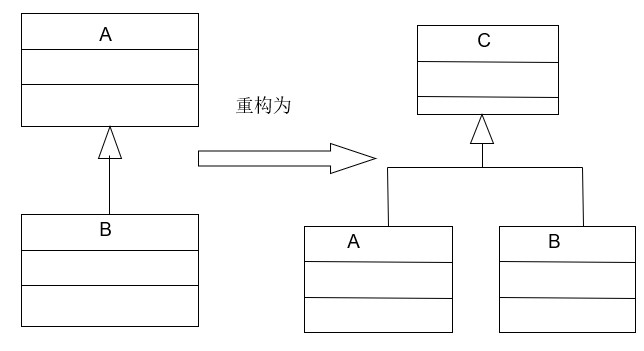
\includegraphics[width=0.55\textwidth]{10_1.jpg}
\end{figure}
下面介绍一个判断正方形是否是长方形的问题.一个长方形(Rectangle)类和正方形(Square)类的代码如下:
\begin{lstlisting}[language=java]
public class Rectangle{
...
  void setWidth(int width){
      this.width=width;
   }
  void setHeight(int height){
      this.height=height
   }
}
\end{lstlisting}
\begin{lstlisting}[language=java]
public class Square{
...
  void setWidth(int width){
      this.width=width;
      this. height=width;
  }
  void setHeight(int height){
      this.setWidth(height);
  }
}
\end{lstlisting}
假设有如下函数,需要对长方形对象的边长进行改动:
\begin{lstlisting}[language=java]
public void resize(Rectangle r){
  while(r.getHeight()<=r.getWidth()){
    r.setHeight(r.getWidth()+1);
  }
}
\end{lstlisting}
如果将正方形作为长方形的子类,这样,只要width或height被赋值,那么width和height会同时赋值,从而长方形的长和宽总是一样的.
换言之,里氏代换原则就被破坏了.
Rectangle和Square都应该同属于四边形(Quadrangle)类的子类,如下图所示:
\begin{figure}[H]
  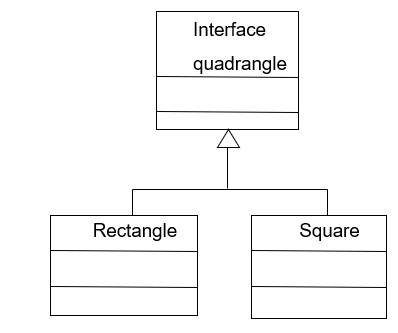
\includegraphics[width=0.35\textwidth]{10_2.jpg}
\end{figure}
\textbf{从B到A的继承关系改为委派delegate关系},如下图:
\begin{figure}[H]
  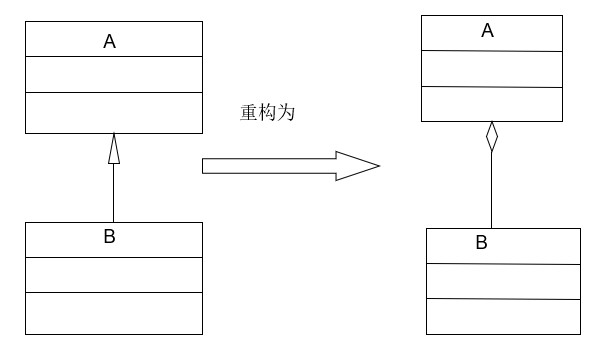
\includegraphics[width=0.40\textwidth]{10_3.jpg}
\end{figure}
\begin{lstlisting}[language=java]
class A {
  void method1();
  void method2() {
    b.method2();
  }
  B b;
}
class B {
  void method2();
}
\end{lstlisting}
从``员工''类派生出``经理''、``总监''、``组长''、``职员''等:
\begin{figure}[H]
  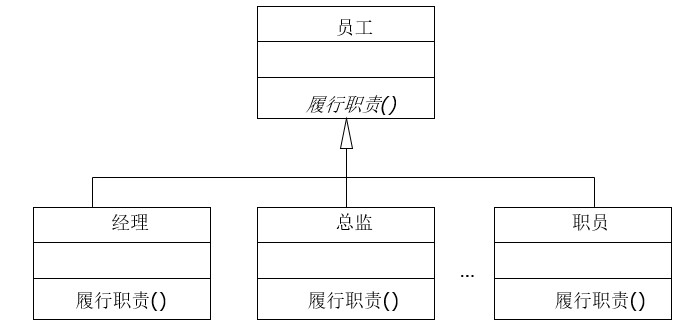
\includegraphics[width=0.50\textwidth]{10_4.jpg}
  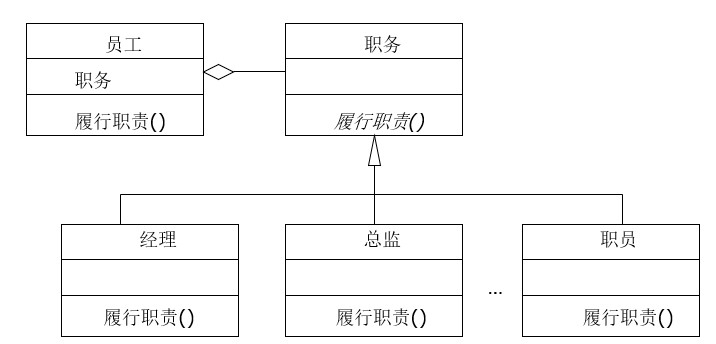
\includegraphics[width=0.50\textwidth]{10_5.jpg}
\end{figure}
将不恰当的继承关系改为组合/聚合关系。将``职务''作为``员工''的一个成员:
\end{document}
